\documentclass[12pt]{article}

\usepackage{sbc-template}
\usepackage{graphicx,url}
\usepackage[utf8]{inputenc}
\usepackage[brazil]{babel}
\usepackage{booktabs}
\usepackage{array}
\usepackage{placeins}
\usepackage{iftex}
\ifXeTeX
  % Compilacao local com tectonic/XeTeX; no Overleaf (pdfLaTeX) este bloco e ignorado.
  \usepackage{fontspec}
  \setmainfont{Times New Roman}
  \setsansfont{Helvetica}
  \setmonofont{Courier New}
\fi
\graphicspath{{figuras/}}
\renewcommand{\topfraction}{0.92}
\renewcommand{\bottomfraction}{0.6}
\renewcommand{\textfraction}{0.06}
\renewcommand{\floatpagefraction}{0.85}
\setcounter{topnumber}{3}
\setcounter{totalnumber}{4}

\sloppy

\title{Previsão da severidade de ocorrências aeronáuticas \\ na aviação comercial brasileira (RBAC 121 e 135)}

\author{Eric I. W. Chou, João Fontanezi, Marcos R. da S. Santos}

\address{Escola de Artes, Ciências e Humanidades -- Universidade de São Paulo
  (EACH -- USP) \\
  \email{choueric24@usp.br, joaofontanezi@usp.br, marcos.santos741e@usp.br}
}

\begin{document}

\maketitle

\begin{resumo}
A aviação comercial brasileira, regida pelos regulamentos RBAC 121 e RBAC 135, opera sob elevados padrões de segurança; ainda assim, incidentes e acidentes aeronáuticos continuam a ocorrer e demandam monitoramento sistemático. O repositório público do Painel SIPAER, mantido pelo Centro de Investigação e Prevenção de Acidentes Aeronáuticos (CENIPA), concentra um extenso histórico de ocorrências, mas sua análise tradicional é retrospectiva e pontual. Este trabalho desenvolve e compara modelos de Aprendizado de Máquina (Regressão Logística multinomial e Random Forest) para classificar a severidade de ocorrências aeronáuticas nas três classes definidas pelo CENIPA (incidente, incidente grave e acidente), usando apenas atributos disponíveis antes da investigação. A base, construída a partir dos dados abertos do CENIPA, reúne 5.038 ocorrências do transporte aéreo comercial entre 2016 e 2026, das quais 91 acidentes (1,8\%) e 102 incidentes graves (2,0\%). Quatro estratégias de balanceamento foram comparadas por validação cruzada estratificada. O Random Forest com SMOTENC obteve F1-macro de 0,62, identificando 60\% dos acidentes e 43\% dos incidentes graves fora da amostra, com AUC de 0,95 para a classe acidente; a Regressão Logística alcançou F1-macro de 0,56. Tipo de operação, peso da aeronave, fase do voo, local e categoria do tipo de ocorrência foram os atributos mais informativos.

\noindent Palavras-chave: Aprendizado de Máquina; Segurança da Aviação; SIPAER; Classificação de Severidade; Regressão Logística; Random Forest.
\end{resumo}

\section{Introdução}
\label{sec:intro}

A segurança operacional na aviação comercial representa um pilar fundamental para o transporte aéreo moderno, exigindo elevados padrões regulatórios, processos contínuos de manutenção e rigorosas rotinas de investigação preventiva. No contexto brasileiro, o transporte aéreo público de passageiros e cargas, regido pelos Regulamentos Brasileiros da Aviação Civil RBAC 121 e RBAC 135, opera sob parâmetros consolidados de confiabilidade e controle de riscos. Ainda assim, a ocorrência contínua de incidentes e acidentes demonstra a permanência de vulnerabilidades operacionais, ambientais e humanas que demandam monitoramento sistemático e estratégias analíticas capazes de auxiliar na gestão da segurança aérea.

O repositório público do Painel SIPAER, mantido pelo Centro de Investigação e Prevenção de Acidentes Aeronáuticos (CENIPA), reúne um volume expressivo de dados históricos referentes a ocorrências, fatores contribuintes e recomendações de segurança aplicadas ao setor aeronáutico nacional. Contudo, a abordagem analítica tradicional aplicada a esse conjunto de informações concentra-se predominantemente na avaliação retrospectiva e pontual de cada evento isolado. Essa característica limita o uso dos registros históricos como um instrumento dinâmico para a identificação de padrões e a antecipação de riscos operacionais. A literatura existente no setor frequentemente prioriza a análise descritiva ou modelos focados em séries temporais agregadas, deixando uma lacuna no que tange ao desenvolvimento de sistemas preditivos capazes de mapear a severidade de novos eventos a partir da combinação multidimensional de atributos operacionais, geográficos e técnicos.

O CENIPA classifica cada ocorrência notificada em três classes, definidas na NSCA 3-13 \cite{brasil:nsca313}. \textbf{Acidente aeronáutico} é toda ocorrência relacionada à operação de uma aeronave, entre o embarque da primeira pessoa com intenção de voo e o desembarque da última, em que uma pessoa sofra lesão grave ou morra, a aeronave sofra dano ou falha estrutural que afete sua resistência, desempenho ou características de voo ou exija grande reparo, ou a aeronave seja considerada desaparecida ou inacessível; excetuam-se danos localizados, como os limitados a um único motor, a hélices e pneus ou os causados por colisão com fauna. \textbf{Incidente aeronáutico} é toda ocorrência, no mesmo intervalo, que não se caracterize como acidente, mas que afete ou possa afetar a segurança da operação. \textbf{Incidente grave} é o incidente cujas circunstâncias indiquem elevado potencial de risco de acidente; a diferença entre ambos está apenas nas consequências.

Para preencher essa lacuna, este trabalho tem como objetivo geral desenvolver e comparar modelos de Aprendizado de Máquina para classificar a severidade das ocorrências na aviação comercial brasileira nas três classes adotadas pelo CENIPA, incidente, incidente grave e acidente, e estimar as probabilidades de cada classe com base nos dados do SIPAER registrados ao longo dos últimos dez anos. Entre os objetivos específicos, destacam-se a estruturação do pipeline de pré-processamento dos dados do CENIPA, a identificação e exclusão dos atributos que só existem após a investigação e que revelariam a própria classe ao modelo, a comparação de técnicas para mitigar o desbalanceamento entre as classes e a avaliação comparativa dos algoritmos de Regressão Logística e Random Forest por meio de métricas direcionadas ao diagnóstico de eventos raros e graves.

A relevância deste estudo reside na oportunidade de transformar registros históricos tabulares em conhecimento preventivo para o setor aéreo. Do ponto de vista prático e operacional, a capacidade de estimar a probabilidade de uma ocorrência configurar um incidente grave ou um acidente permite que órgãos reguladores e companhias aéreas direcionem recursos de fiscalização, treinamento e auditoria para as áreas de maior risco condicional. No âmbito acadêmico, a pesquisa contribui ao demonstrar a aplicação de modelos discriminativos em bases de dados públicas da aviação civil nacional, validando estratégias de tratamento de desequilíbrio de dados em cenários de alta gravidade.

O restante deste artigo está organizado como segue. A Seção~\ref{sec:correlatos} apresenta a revisão dos trabalhos correlatos, com uma tabela comparativa, e destaca a diferença da abordagem proposta em relação às pesquisas anteriores. A Seção~\ref{sec:metodo} detalha a metodologia adotada, abrangendo a fonte dos dados, as definições das classes, o recorte amostral, o pré-processamento, os algoritmos e a estratégia de validação. A Seção~\ref{sec:resultados} reporta os resultados parciais: a caracterização da base e a avaliação de desempenho dos classificadores. Por fim, a Seção~\ref{sec:conclusao} traz a discussão sobre os achados, as limitações e os próximos passos.

\section{Trabalhos Correlatos}
\label{sec:correlatos}

A literatura dedicada à análise de ocorrências e à prevenção de acidentes na aviação civil brasileira fundamenta-se, predominantemente, em abordagens estatísticas descritivas, modelos de séries temporais agregadas e investigações focadas em fatores ambientais isolados. Diversos estudos buscam mapear o comportamento histórico de eventos aeronáuticos a fim de identificar tendências temporais ou compreender o impacto de variáveis meteorológicas sobre a segurança de voo, provendo diagnósticos relevantes para o setor.

\begin{table}[tbp]
    \centering
    \caption{Comparação entre os trabalhos correlatos e este trabalho}
    \vspace{0.2cm}
    \footnotesize\setlength{\tabcolsep}{4pt}
    \begin{tabular}{>{\raggedright\arraybackslash}p{2.2cm}>{\raggedright\arraybackslash}p{3.1cm}>{\raggedright\arraybackslash}p{3.5cm}>{\raggedright\arraybackslash}p{4.9cm}}
        \toprule
        \textbf{Referência} & \textbf{Modelo} & \textbf{Dados utilizados} & \textbf{Contribuição deste trabalho} \\
        \midrule
        Reinert (2023) &
        Ajuste de curvas e modelos auto-regressivos (ARIMA) sobre séries anuais agregadas de acidentes, fatalidades e taxas de mortalidade &
        Ocorrências do SIPAER entre 2012 e 2022 com aviões Ipanema (agrícola) e Sêneca (aviação geral), agregadas por ano &
        Classifica a severidade de cada ocorrência individual em três classes a partir de atributos pré-investigação, em vez de projetar volumes agregados; cobre todo o transporte aéreo comercial (RBAC 121 e 135), não dois modelos de aeronave \\
        \midrule
        Soares (2012) &
        Análise sinótica qualitativa (cartas meteorológicas e imagens de satélite) de casos selecionados &
        Acidentes aéreos no Brasil na década de 1990 associados a condições meteorológicas adversas, com registros do CENIPA e dados meteorológicos &
        Quantifica o risco por modelos discriminativos que combinam operação, aeronave, fase do voo, local e tipo de ocorrência, com a meteorologia como uma das categorias de tipo; estimativa probabilística validada por métricas, em vez de descrição de casos \\
        \midrule
        Barros e Balero (2012) &
        Pesquisa bibliográfica e estatística descritiva &
        Dados de estações meteorológicas do Centro-Oeste e estatísticas descritivas do SIPAER &
        Abrangência nacional, com a região como preditor entre outros atributos; avaliação fora da amostra por validação cruzada e conjunto de teste, com baselines explícitos \\
        \bottomrule
    \end{tabular}
    \label{tab:correlatos}
\end{table}

Entre as abordagens orientadas à modelagem preditiva temporal, destaca-se o estudo de Reinert \cite{reinert:2023}, que analisou as ocorrências registradas no SIPAER entre 2012 e 2022 para as aeronaves Ipanema e Sêneca. Utilizando técnicas de ajuste de curvas e modelos auto-regressivos do tipo ARIMA, o autor buscou prever tendências futuras de acidentes, fatalidades e taxas de mortalidade para esses modelos específicos. Embora a modelagem temporal agregada seja eficaz para projetar volumes globais de eventos em janelas futuras, esse método avalia o risco de forma genérica e agregada ao longo do tempo, sem capacidade de classificar a severidade ou o risco condicional de uma ocorrência individual a partir de suas características técnicas e operacionais imediatas.

Por outro lado, vertentes da literatura priorizam a influência de variáveis ambientais e meteorológicas sobre a ocorrência de eventos severos. Soares \cite{soares:2012} investigou a relação entre condições meteorológicas adversas e acidentes aéreos no Brasil durante a década de 1990 por meio de análises sinóticas, exemplificando como a interação de sistemas atmosféricos de grande escala pode intensificar fenômenos convectivos e degradar as condições de voo. De forma complementar, Barros e Balero \cite{barros:2012} examinaram o impacto das características climáticas do Centro-Oeste brasileiro nas condições operacionais de voo, combinando pesquisa bibliográfica, dados de estações meteorológicas e estatísticas descritivas do SIPAER para ressaltar a importância da consciência meteorológica na formação de pilotos e no planejamento de voo. Ambos os trabalhos oferecem contribuições qualitativas valiosas para a compreensão dos fatores determinantes do risco ambiental, porém adotam uma perspectiva predominantemente descritiva e não estruturam modelos preditivos capazes de quantificar probabilisticamente o risco de evolução de um evento para acidente.

A Tabela~\ref{tab:correlatos} sintetiza a comparação. Em contraste com os trabalhos analisados, a abordagem proposta neste artigo diferencia-se em três eixos centrais: a natureza do modelo, o escopo dos dados e o foco na decisão operacional. Enquanto os estudos anteriores priorizam séries temporais agregadas para modelos específicos de aeronaves \cite{reinert:2023} ou análises qualitativo-descritivas do fator meteorológico \cite{soares:2012,barros:2012}, este trabalho desenvolve um arcabouço preditivo discriminativo baseado em Aprendizado de Máquina (Regressão Logística e Random Forest) que estima, para cada ocorrência individual, a probabilidade de ela configurar um incidente, um incidente grave ou um acidente, a partir da combinação de atributos operacionais, geográficos e técnicos disponíveis antes da investigação. Além disso, ao restringir o escopo ao transporte aéreo comercial (RBAC 121 e RBAC 135), tratar explicitamente o vazamento de informação produzido pela investigação e comparar técnicas de balanceamento para eventos raros, este estudo avança em relação à literatura ao transformar registros históricos abertos em um modelo classificatório com aplicação prática na gestão preventiva de riscos aeronáuticos.


\section{Metodologia}
\label{sec:metodo}

    \subsection{Fonte de dados, definições das classes e recorte amostral}
    \label{sec:fonte}

    Este estudo quantitativo e observacional retrospectivo utiliza os dados abertos de ocorrências aeronáuticas do CENIPA \cite{cenipa:ocorrencias,cenipa:painelsipaer}, nos dez anos anteriores ao registro mais recente dos arquivos (10/05/2016 a 09/05/2026).

    A variável alvo é a classificação atribuída pelo CENIPA a cada ocorrência, nas três classes definidas na Seção~\ref{sec:intro}. As três classes são mantidas separadas, sem agrupar os incidentes graves aos incidentes ou aos acidentes: as definições distinguem o incidente grave pelo potencial de risco, e não pela consequência, e a análise exploratória (Seção~\ref{sec:tipos}) mostra que incidentes graves e acidentes têm perfis distintos. Agrupá-los ocultaria a classe de maior valor preventivo, a dos quase-acidentes.

    O recorte manteve as ocorrências com ao menos uma aeronave em operação regular, não regular ou de táxi aéreo, que correspondem ao transporte aéreo público regido pelo RBAC 121 (aviões com mais de 19 assentos ou carga paga acima de 3.400 kg) e pelo RBAC 135 (aviões de até 19 assentos ou helicópteros) \cite{anac:rbac121,anac:rbac135}, excluindo a aviação geral, de instrução, agrícola e experimental. O táxi aéreo e a operação não regular integram o escopo ao lado da operação regular porque pertencem à mesma família regulatória, porque a operação regular isolada registra apenas 12 acidentes e 43 incidentes graves no período, insuficiente para aprendizado supervisionado, e porque o tipo de operação entra como preditor, capturando a diferença de risco entre os segmentos.

    \subsection{Construção da base, atributos e vazamento de informação}
    \label{sec:atributos}

    As tabelas de Ocorrências, Tipos de Ocorrência, Aeronaves, Fatores Contribuintes e Recomendações foram cruzadas pelo código da ocorrência, resultando em uma linha por ocorrência com os atributos da aeronave comercial envolvida; os marcadores de ausência do CENIPA (``***'', ``NULL'', ``INDETERMINADO'', ``DESCONHECIDO'') foram convertidos em nulos. Os preditores restringem-se às informações disponíveis no momento da notificação: tipo de operação, tipo de equipamento, tipo e quantidade de motores, fabricante, peso máximo de decolagem (em escala logarítmica), número de assentos, idade da aeronave, fase do voo (quatro grupos), região, local (aeródromos de código SB, demais aeródromos ou fora de aeródromo), categoria do tipo de ocorrência (65 tipos em sete categorias), número de tipos atribuídos, indicador de saída de pista, número de aeronaves envolvidas, mês, dia da semana e hora.

    Os atributos produzidos pela investigação (nível de dano, fatalidades, situação da investigação, relatório final, fatores contribuintes e recomendações) permanecem na base para a análise descritiva, mas não são usados como preditores: a investigação completa é conduzida quase apenas em acidentes e incidentes graves, e esses atributos revelariam a própria classe ao modelo (Seção~\ref{sec:alvo}). O ano também não é usado, pela mudança de cobertura das notificações a partir de 2023 (Seção~\ref{sec:temporal}). O código do aeródromo (203 níveis) e o tipo detalhado (65 níveis) foram substituídos pelos seus agrupamentos; a codificação pelo alvo fica como trabalho futuro, pois com 91 acidentes tende a introduzir ruído. Valores faltantes são imputados pela mediana (numéricos) ou pela moda (categóricos), e os categóricos são codificados por variáveis indicadoras; imputação, padronização e codificação são ajustadas apenas nas dobras de treino, evitando vazamento para os dados avaliados.

    \subsection{Algoritmos, balanceamento e protocolo de avaliação}
    \label{sec:protocolo}

    Dois algoritmos supervisionados foram implementados e comparados: a \textbf{Regressão Logística multinomial}, modelo linear de referência que estima as probabilidades das três classes e permite interpretar o peso de cada atributo por razões de chance (regularização L2, $C$ entre 0,01 e 10); e o \textbf{Random Forest} \cite{breiman:2001}, \textit{ensemble} não linear de 400 árvores, capaz de capturar interações entre atributos (profundidade, folha mínima e atributos por divisão escolhidos por validação cruzada).

    Para o desbalanceamento, quatro estratégias foram comparadas: nenhuma; pesos de classe inversamente proporcionais à frequência; sobreamostragem sintética das classes minoritárias com SMOTENC \cite{chawla:2002}, variante do SMOTE para dados mistos que preserva as variáveis categóricas, aplicada apenas às dobras de treino; e SMOTENC combinado a pesos. Como o SMOTENC iguala as frequências das classes, os pesos balanceados calculados em seguida são unitários e a quarta estratégia equivale à terceira; ela foi incluída como verificação dessa redundância.

    A base foi particionada de forma estratificada em 80\% para treinamento (4.030 ocorrências: 3.876 incidentes, 81 incidentes graves e 73 acidentes) e 20\% para teste (1.008: 969, 21 e 18). Os hiperparâmetros de cada combinação foram escolhidos por busca em grade com validação cruzada estratificada ($k = 5$) no treino, maximizando o F1-macro. Como o teste contém apenas 18 acidentes, em que cada erro desloca a sensibilidade em 5,6 pontos percentuais, as predições \textit{out-of-fold} da validação cruzada no treino são o resultado principal, e o teste, a confirmação. A classe prevista é a de maior probabilidade; o ajuste de limiares fica para a etapa final. Dois baselines dão escala aos resultados: a classe majoritária e a regra ``táxi aéreo ou operação não regular implica acidente; caso contrário, incidente''. O pipeline usa Python, scikit-learn \cite{pedregosa:2011} e imbalanced-learn \cite{lemaitre:2017}; código, base e dicionário estão no repositório do projeto\footnote{\url{https://github.com/Fontanezi/RP2_ARTIGO_2026}}.

    \subsection{Métricas de avaliação de desempenho}
    \label{sec:metricas}

    A acurácia é reportada apenas como referência, pois prever sempre a classe majoritária acerta 96,2\% dos casos. O desempenho é mensurado por: sensibilidade (\textit{recall}), precisão e F1 por classe, com prioridade para a sensibilidade nas classes acidente e incidente grave, a fim de minimizar falsos negativos; F1-macro, média dos F1 das três classes, usado como critério de seleção; acurácia balanceada, média das sensibilidades; AUC-ROC um-contra-resto, que avalia a ordenação das probabilidades; precisão média (AP) da curva precisão-sensibilidade, mais informativa que a ROC com prevalência de 2\%; e matriz de confusão $3 \times 3$. A interpretação usa os coeficientes da Regressão Logística, como log da razão de chances entre acidente e incidente em relação ao nível mais frequente de cada atributo, e a importância por permutação do Random Forest no teste (queda da AUC um-contra-resto, 30 repetições).

\section{Resultados Parciais}
\label{sec:resultados}

\subsection{Construção e caracterização da base}
\label{sec:base}

A base foi construída conforme a Seção~\ref{sec:atributos}: dos 14.626 registros dos arquivos do CENIPA, 9.471 estão na janela de dez anos e 5.038 envolvem ao menos uma aeronave em operação comercial. Cada linha corresponde a uma ocorrência; nas 46 com duas aeronaves comerciais, manteve-se a primeira listada, e o código da ocorrência é único na base final. A omissão é inferior a 1\% em todos os atributos categóricos candidatos a preditor e mais alta apenas no número de assentos (10,2\%) e no ano de fabricação (14,2\%); como a imputação é ajustada somente no treino, os nulos foram mantidos na base publicada (BASE\_SIPAER.xlsx, 5.038 linhas e 44 colunas, acompanhada de dicionário de dados).

\subsection{Classes e atributos posteriores ao evento}
\label{sec:alvo}

A base contém 91 acidentes (1,81\%), 102 incidentes graves (2,02\%) e 4.845 incidentes (96,2\%). Dos acidentes, 17 tiveram vítimas fatais, somando 122 mortes, 62 delas no acidente de Vinhedo (SP), em 09/08/2024; nenhum incidente grave registrou fatalidade, o que é coerente com a definição da classe.

Vários atributos das tabelas cruzadas só existem porque a ocorrência foi investigada, e a investigação completa é feita quase apenas para acidentes e incidentes graves. A Tabela~\ref{tab:posevento} mostra o efeito: o relatório final, os fatores contribuintes e as recomendações aparecem em 61\% a 68\% dos acidentes e em 44\% a 45\% dos incidentes graves, mas em 0,1\% dos incidentes. Usá-los como preditores entregaria ao modelo a própria resposta; o mesmo vale para o nível de dano, que integra a definição de acidente (92\% dos acidentes com dano substancial ou aeronave destruída, contra 2\% dos incidentes graves). Entre os 56 acidentes com fatores registrados, 54 têm fatores da área operacional e 46 da área humana; os mais frequentes são processo decisório (25), julgamento de pilotagem (24) e supervisão gerencial (20). Nos 45 incidentes graves com fatores, predominam percepção (20), atenção (19) e atitude (19). Esses resultados caracterizam as ocorrências já investigadas, mas não antecipam a severidade de uma ocorrência nova.

\begin{table}[htbp]
    \centering
    \caption{Atributos produzidos pela investigação, por classe}
    \vspace{0.2cm}
    \footnotesize\setlength{\tabcolsep}{3.5pt}
    \begin{tabular}{lccc}
\toprule
\textbf{Atributo} & \textbf{Acidentes (91)} & \textbf{Inc. graves (102)} & \textbf{Incidentes (4.845)} \\
\midrule
Dano substancial ou aeronave destruída & 84 (92,3\%) & 2 (2,0\%) & 2 (0,0\%) \\
Relatório final publicado & 62 (68,1\%) & 46 (45,1\%) & 5 (0,1\%) \\
Fatores contribuintes registrados & 56 (61,5\%) & 45 (44,1\%) & 4 (0,1\%) \\
Recomendações de segurança emitidas & 19 (20,9\%) & 29 (28,4\%) & 1 (0,0\%) \\
Investigação ainda ativa & 28 (30,8\%) & 30 (29,4\%) & 7 (0,1\%) \\
\bottomrule
\end{tabular}
    \label{tab:posevento}
\end{table}

\subsection{Operação e características da aeronave}
\label{sec:operacao}

O tipo de operação é o atributo que mais separa as classes (Tabela~\ref{tab:operacao}). A operação regular responde por 85,4\% das ocorrências, mas por apenas 12 acidentes (0,28\%) e 43 incidentes graves (1,0\%); o táxi aéreo, com 12,9\% das ocorrências, concentra 72 dos 91 acidentes (11,1\%) e 50 incidentes graves (7,7\%), e a operação não regular tem as maiores taxas de incidente grave (10,2\%). As características da aeronave seguem o mesmo padrão: a taxa de acidentes é de 22,6\% em aeronaves a pistão contra 0,32\% nos jatos, de 15,9\% nas monomotoras e de 7,5\% nos helicópteros. Airbus e Boeing somam 2.897 ocorrências, 30 incidentes graves e 8 acidentes; Cessna e Robinson somam 239 ocorrências, 19 incidentes graves e 32 acidentes. As medianas de idade e de peso máximo de decolagem ordenam as classes: 11 anos e 70,5 t nos incidentes, 16 anos e 7,3 t nos incidentes graves e 32 anos e 2,2 t nos acidentes.

\begin{table}[htbp]
    \centering
    \caption{Incidentes graves e acidentes por tipo de operação, características da aeronave e fase do voo}
    \vspace{0.2cm}
    \footnotesize\setlength{\tabcolsep}{5pt}
    \begin{tabular}{lccccc}
\toprule
\textbf{Atributo} & \textbf{Ocorrências} & \textbf{Inc. graves} & \textbf{Acidentes} & \textbf{\% inc. graves} & \textbf{\% acidentes} \\
\midrule
\multicolumn{6}{l}{\textit{Tipo de operação}} \\
\hspace{1em}Regular & 4.302 & 43 & 12 & 1,00 & 0,28 \\
\hspace{1em}Não regular & 88 & 9 & 7 & 10,23 & 7,95 \\
\hspace{1em}Táxi aéreo & 648 & 50 & 72 & 7,72 & 11,11 \\
\multicolumn{6}{l}{\textit{Tipo de motor}} \\
\hspace{1em}Jato & 3.702 & 43 & 12 & 1,16 & 0,32 \\
\hspace{1em}Turboélice & 775 & 19 & 17 & 2,45 & 2,19 \\
\hspace{1em}Turboeixo & 352 & 10 & 17 & 2,84 & 4,83 \\
\hspace{1em}Pistão & 199 & 29 & 45 & 14,57 & 22,61 \\
\multicolumn{6}{l}{\textit{Equipamento}} \\
\hspace{1em}Avião & 4.610 & 91 & 62 & 1,97 & 1,34 \\
\hspace{1em}Helicóptero & 375 & 11 & 28 & 2,93 & 7,47 \\
\multicolumn{6}{l}{\textit{Fase do voo}} \\
\hspace{1em}Solo & 547 & 6 & 0 & 1,10 & 0,00 \\
\hspace{1em}Decolagem e subida & 1.651 & 16 & 19 & 0,97 & 1,15 \\
\hspace{1em}Cruzeiro e descida & 1.027 & 14 & 28 & 1,36 & 2,73 \\
\hspace{1em}Aproximação e pouso & 1.770 & 66 & 42 & 3,73 & 2,37 \\
\bottomrule
\end{tabular}
    \label{tab:operacao}
\end{table}

Esses atributos não são independentes: o táxi aéreo reúne 153 das 199 aeronaves a pistão e 266 dos 375 helicópteros, além de aeronaves mais leves e antigas. Na Regressão Logística, essa correlação torna instáveis as razões de chance de cada atributo isolado, que devem ser lidas em conjunto; o Random Forest é menos sensível a isso. Quanto à fase do voo, nenhuma das 547 ocorrências em solo resultou em acidente, as taxas de acidente são maiores no cruzeiro e descida (2,73\%) e na aproximação e pouso (2,37\%), e os incidentes graves concentram-se na aproximação e pouso, com 66 dos 102 casos (3,73\%).

\subsection{Tipos de ocorrência}
\label{sec:tipos}

Os 65 tipos de ocorrência foram agrupados em sete categorias; nas 80 ocorrências com mais de um tipo, prevaleceu o mais próximo da perda da aeronave (perda de controle ou colisão em voo, pista, pouso e solo, tráfego aéreo, meteorologia, fauna e falha técnica, nesta ordem). A Tabela~\ref{tab:tipos_ocorrencia} apresenta o resultado.

\begin{table}[htbp]
    \centering
    \caption{Ocorrências, incidentes graves e acidentes por categoria de tipo}
    \vspace{0.2cm}
    \footnotesize\setlength{\tabcolsep}{3pt}
    \begin{tabular}{lcccccc}
\toprule
\textbf{Categoria} & \textbf{Ocorrências} & \textbf{\%} & \textbf{Inc. graves} & \textbf{\% inc. gr.} & \textbf{Acidentes} & \textbf{\% acid.} \\
\midrule
Falha técnica & 2.512 & 49,9 & 29 & 1,15 & 34 & 1,35 \\
Colisão com fauna & 1.767 & 35,1 & 0 & 0,00 & 1 & 0,06 \\
Pista, pouso e solo & 323 & 6,4 & 41 & 12,69 & 32 & 9,91 \\
Tráfego aéreo & 193 & 3,8 & 21 & 10,88 & 0 & 0,00 \\
Meteorologia & 94 & 1,9 & 1 & 1,06 & 3 & 3,19 \\
Perda de controle / colisão em voo & 20 & 0,4 & 5 & 25,00 & 12 & 60,00 \\
Outros & 129 & 2,6 & 5 & 3,88 & 9 & 6,98 \\
\midrule
\textbf{Total} & \textbf{5.038} & \textbf{100,0} & \textbf{102} & \textbf{2,02} & \textbf{91} & \textbf{1,81} \\
\bottomrule
\end{tabular}
    \label{tab:tipos_ocorrencia}
\end{table}

Falhas técnicas e colisões com fauna somam 84,9\% das ocorrências, mas as colisões com fauna quase nunca evoluem para incidente grave ou acidente (0 e 1 em 1.767). Dentro das falhas técnicas, os acidentes concentram-se na falha do motor em voo (14 acidentes e nenhum incidente grave em 122 registros). Perda de controle ou colisão em voo (60,0\% de acidentes e 25,0\% de incidentes graves) e pista, pouso e solo (9,9\% e 12,7\%) têm as maiores taxas; as 62 ocorrências com excursão de pista produziram 20 acidentes e 25 incidentes graves. O tráfego aéreo não registra acidentes, mas reúne 21 incidentes graves (10,9\%), em geral conflitos entre duas aeronaves. Os perfis diferem: falha do motor em voo e perda de controle levam ao acidente; tráfego aéreo e ocorrências em pista geram incidentes graves, o que sustenta a formulação em três classes (Seção~\ref{sec:fonte}).

\subsection{Distribuição temporal e geográfica}
\label{sec:temporal}

A Figura~\ref{fig:temporal} mostra uma descontinuidade a partir de 2023: de 2016 a 2022 há 1.097 ocorrências, e de 2023 a 2026, 3.941, com pico de 1.582 em 2024. O aumento está quase todo na operação regular e nas colisões com fauna (1.462 registros só em 2023 e 2024), enquanto os números anuais de incidentes graves e de acidentes não crescem; suas proporções caem de 5,8\% e 5,9\% antes de 2023 para 1,0\% e 0,7\% depois, o que é compatível com uma ampliação da notificação de incidentes, e não com uma queda real do risco. Há também defasagem de registro nos meses recentes (o táxi aéreo tem 188 ocorrências em 2025 e 8 em 2026); por isso, o ano é usado apenas como controle.

\begin{figure}[htbp]
    \centering
    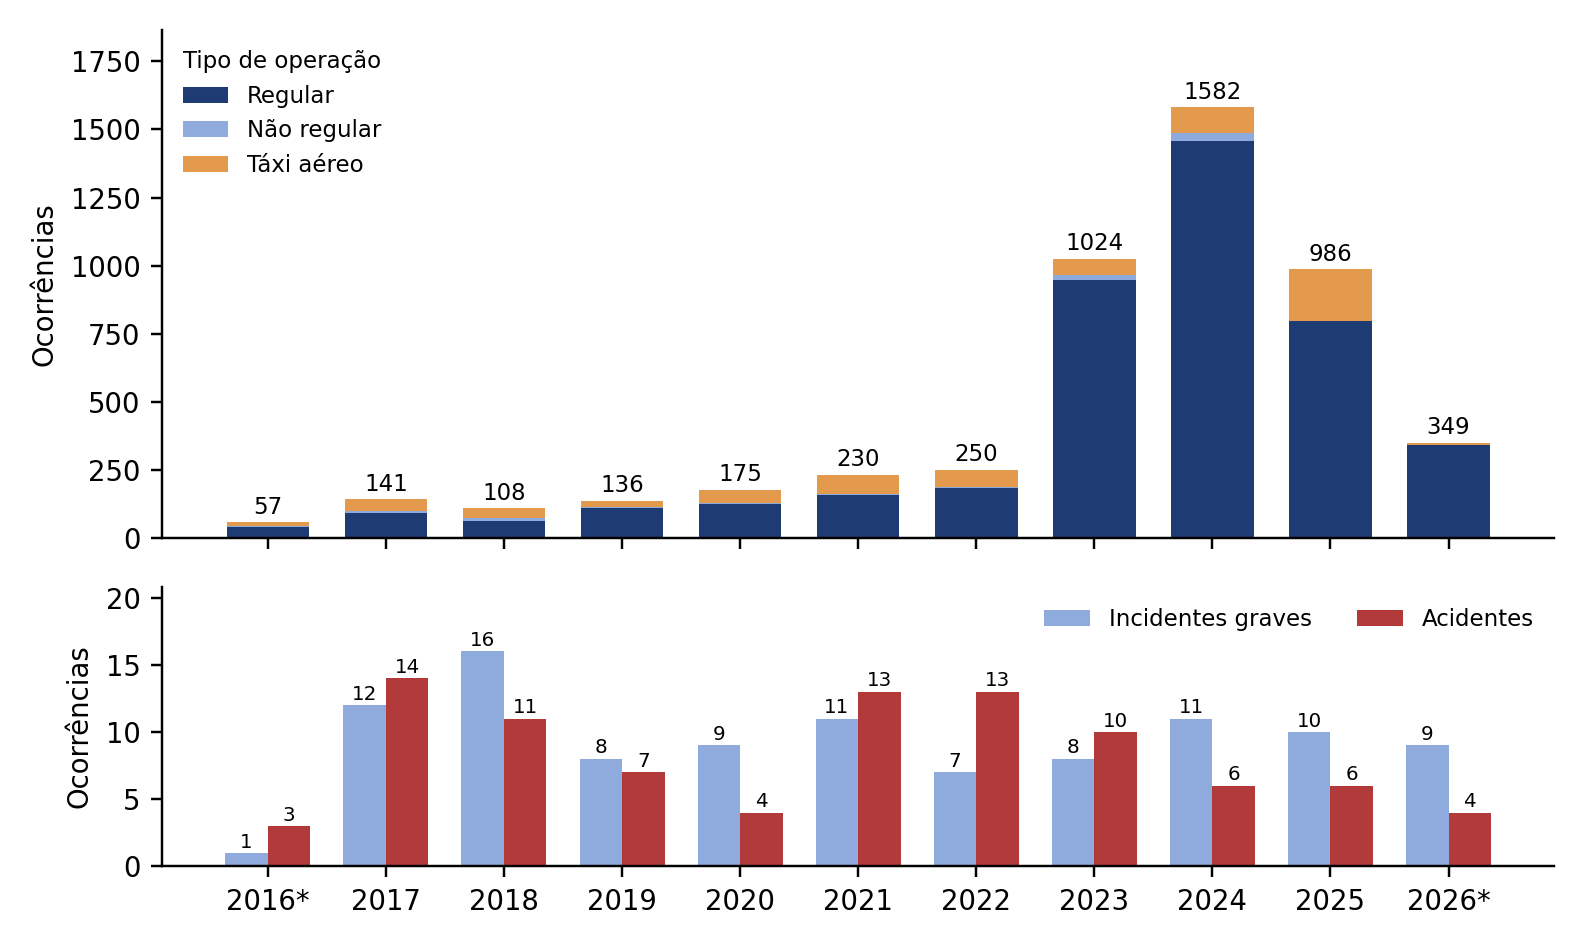
\includegraphics[width=0.6\textwidth]{fig1_anual.png}
    \caption{Ocorrências por ano e tipo de operação (acima) e incidentes graves e acidentes por ano (abaixo); * 2016 e 2026 parciais}
    \label{fig:temporal}
\end{figure}

Na distribuição geográfica (Figura~\ref{fig:geografica}a), o Sudeste concentra 50,9\% das ocorrências e tem taxas de 1,1\% de incidentes graves e 0,8\% de acidentes, enquanto o Norte, com 10,5\% das ocorrências, responde por 32 incidentes graves (6,0\%) e 44 dos 91 acidentes (8,3\%). O contraste também reflete a operação: 35\% das ocorrências do Norte são de táxi aéreo, contra 13\% no país. O local da ocorrência (Figura~\ref{fig:geografica}b) separa as duas classes graves: os aeródromos de código SB, em geral os de maior movimento, reúnem 83,0\% das ocorrências com taxa de acidentes de 0,33\%, mas 57 dos 102 incidentes graves ocorreram neles; já 49 dos 91 acidentes ocorreram fora de aeródromo (8,5\%).

\begin{figure}[htbp]
    \centering
    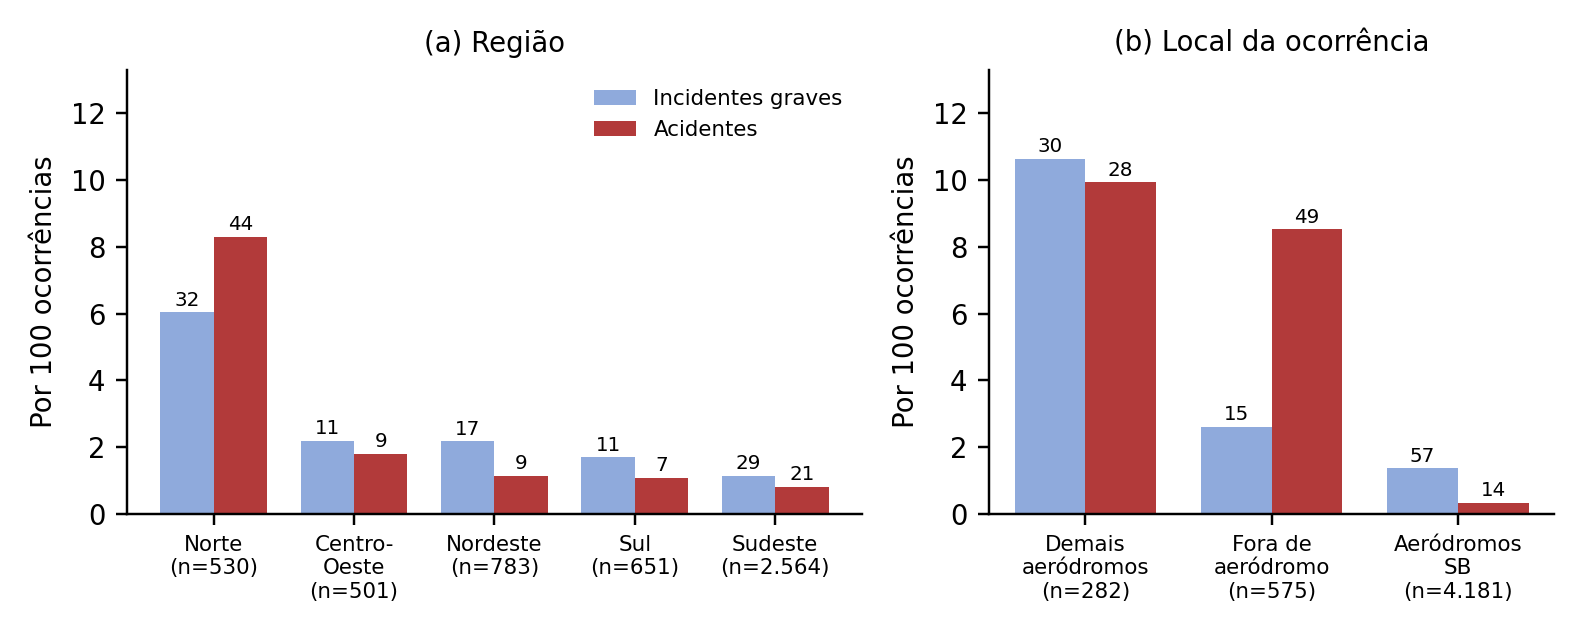
\includegraphics[width=0.72\textwidth]{fig2_regiao_local.png}
    \caption{Incidentes graves e acidentes por 100 ocorrências segundo a região (a) e o local da ocorrência (b); os rótulos indicam as contagens}
    \label{fig:geografica}
\end{figure}

\subsection{Desempenho dos modelos}
\label{sec:desempenho}

A Tabela~\ref{tab:ablacao} compara as estratégias de balanceamento, com o F1-macro da validação cruzada usado na seleção e as métricas \textit{out-of-fold} no treino. O efeito depende do algoritmo. Na Regressão Logística, o F1-macro é maior sem balanceamento (0,556), mas esse modelo detecta apenas 37\% dos acidentes; os pesos de classe elevam a sensibilidade para 71\% dos acidentes e 48\% dos incidentes graves ao custo de precisões de 18\% e 15\%, derrubando o F1-macro para 0,483. No Random Forest, pesos e SMOTENC empatam (0,62) e elevam a sensibilidade para acidentes de 41\% para 60\% a 63\% com precisão em torno de 45\%; o SMOTENC foi escolhido pela menor variância entre dobras, e sua combinação com pesos reproduz exatamente o SMOTENC isolado, como previsto na Seção~\ref{sec:protocolo}.

\begin{table}[htbp]
    \centering
    \caption{Estratégias de balanceamento: F1-macro na validação cruzada (média $\pm$ desvio-padrão entre dobras) e métricas \textit{out-of-fold} no treino, em \%, para acidentes (AC) e incidentes graves (IG); $\dagger$ configuração selecionada}
    \vspace{0.2cm}
    \scriptsize\setlength{\tabcolsep}{3.5pt}
    \begin{tabular}{llcccccc}
\toprule
\textbf{Modelo} & \textbf{Balanceamento} & \textbf{F1-macro CV} & \textbf{Sens. AC} & \textbf{Prec. AC} & \textbf{Sens. IG} & \textbf{Prec. IG} & \textbf{AUC AC} \\
\midrule
Regressão Logística & Nenhum$\dagger$ & 0,556 $\pm$ 0,076 & 37,0 & 46,6 & 21,0 & 48,6 & 0,944 \\
 & Pesos de classe & 0,483 $\pm$ 0,013 & 71,2 & 17,7 & 48,1 & 14,9 & 0,931 \\
 & SMOTENC & 0,513 $\pm$ 0,022 & 64,4 & 22,8 & 49,4 & 16,2 & 0,931 \\
 & SMOTENC + pesos & 0,513 $\pm$ 0,022 & 64,4 & 22,8 & 49,4 & 16,2 & 0,931 \\
\midrule
Random Forest & Nenhum & 0,575 $\pm$ 0,031 & 41,1 & 62,5 & 17,3 & 43,8 & 0,933 \\
 & Pesos de classe & 0,622 $\pm$ 0,020 & 63,0 & 43,4 & 37,0 & 37,5 & 0,953 \\
 & SMOTENC$\dagger$ & 0,623 $\pm$ 0,009 & 60,3 & 45,8 & 43,2 & 33,0 & 0,945 \\
 & SMOTENC + pesos & 0,623 $\pm$ 0,009 & 60,3 & 45,8 & 43,2 & 33,0 & 0,945 \\
\bottomrule
\end{tabular}
    \label{tab:ablacao}
\end{table}

A Tabela~\ref{tab:metricas} reúne os modelos selecionados e os baselines. A classe majoritária alcança 96,2\% de acurácia sem detectar nenhuma ocorrência grave (F1-macro de 0,327). A regra pelo tipo de operação detecta 86\% dos acidentes, mas com precisão de 10,7\% (F1 de 0,19 para a classe) e sem distinguir incidentes graves. O Random Forest com SMOTENC identifica 44 dos 73 acidentes (60\%) com precisão de 46\% (F1 de 0,52) e 35 dos 81 incidentes graves (43\%) com precisão de 33\%, com F1-macro de 0,624 e acurácia balanceada de 0,669; a Regressão Logística identifica 27 acidentes (37\%) e 17 incidentes graves (21\%), com F1-macro de 0,563. O teste confirma a ordem: o Random Forest detecta 11 dos 18 acidentes e 8 dos 21 incidentes graves (F1-macro de 0,609), contra 10, 2 e 0,560 da Regressão Logística. As AUC no teste (0,97 a 0,98 para acidente) superam as da validação cruzada (0,94), diferença compatível com a variância de uma amostra de 18 acidentes.

\begin{table}[htbp]
    \centering
    \caption{Desempenho dos baselines e dos modelos selecionados nas predições \textit{out-of-fold} do treino e no teste; sensibilidade e precisão em \%, para acidentes (AC), incidentes graves (IG) e incidentes (INC)}
    \vspace{0.2cm}
    \scriptsize\setlength{\tabcolsep}{3.5pt}
    \begin{tabular}{lcccccccc}
\toprule
\textbf{Modelo} & \textbf{Sens. AC} & \textbf{Prec. AC} & \textbf{Sens. IG} & \textbf{Prec. IG} & \textbf{Sens. INC} & \textbf{F1-macro} & \textbf{Acur. bal.} & \textbf{AUC AC} \\
\midrule
\multicolumn{9}{l}{\textit{Validação cruzada no treino (73 acidentes, 81 incidentes graves)}} \\
Classe majoritária & 0,0 & 0,0 & 0,0 & 0,0 & 100,0 & 0,327 & 0,333 & -- \\
Regra pelo tipo de operação & 86,3 & 10,7 & 0,0 & 0,0 & 87,7 & 0,373 & 0,580 & -- \\
Regressão Logística (Nenhum) & 37,0 & 46,6 & 21,0 & 48,6 & 99,3 & 0,563 & 0,524 & 0,944 \\
Random Forest (SMOTENC) & 60,3 & 45,8 & 43,2 & 33,0 & 97,2 & 0,624 & 0,669 & 0,945 \\
\midrule
\multicolumn{9}{l}{\textit{Teste (18 acidentes, 21 incidentes graves)}} \\
Classe majoritária & 0,0 & 0,0 & 0,0 & 0,0 & 100,0 & 0,327 & 0,333 & -- \\
Regra pelo tipo de operação & 88,9 & 10,8 & 0,0 & 0,0 & 87,4 & 0,373 & 0,588 & -- \\
Regressão Logística (Nenhum) & 55,6 & 55,6 & 9,5 & 25,0 & 99,4 & 0,560 & 0,548 & 0,981 \\
Random Forest (SMOTENC) & 61,1 & 45,8 & 38,1 & 28,6 & 97,1 & 0,609 & 0,654 & 0,973 \\
\bottomrule
\end{tabular}
    \label{tab:metricas}
\end{table}

As matrizes de confusão (Figura~\ref{fig:confusao}) mostram onde estão os erros. No Random Forest, os acidentes não detectados são previstos sobretudo como incidentes (23) e raramente como incidentes graves (6), e os incidentes graves não detectados dividem-se entre incidente (36) e acidente (10); o custo da sensibilidade são 65 incidentes previstos como graves e 42 como acidentes, 2,8\% dos incidentes. A Regressão Logística quase não prevê a classe incidente grave (35 predições em 4.030), a de sinal mais fraco. As curvas da Figura~\ref{fig:curvas} dão a visão independente do limiar: para a classe acidente, os dois modelos têm AUC de 0,94 e precisão média de 0,41 a 0,44, cerca de 24 vezes a prevalência de 1,8\%; para incidente grave, a AUC cai para 0,85 a 0,88 e a precisão média para 0,23 a 0,33. No mesmo nível de sensibilidade da regra pelo tipo de operação (86\%), marcada nas curvas, a precisão dos modelos para acidentes é de 16,7\% (Regressão Logística) e 13,8\% (Random Forest), contra 10,7\% da regra: o ganho existe, mas é modesto nesse ponto de operação. A vantagem dos modelos concentra-se na faixa intermediária, em que o Random Forest mantém precisão de 45\% a 70\% com sensibilidade de 40\% a 65\%.

\begin{figure}[htbp]
    \centering
    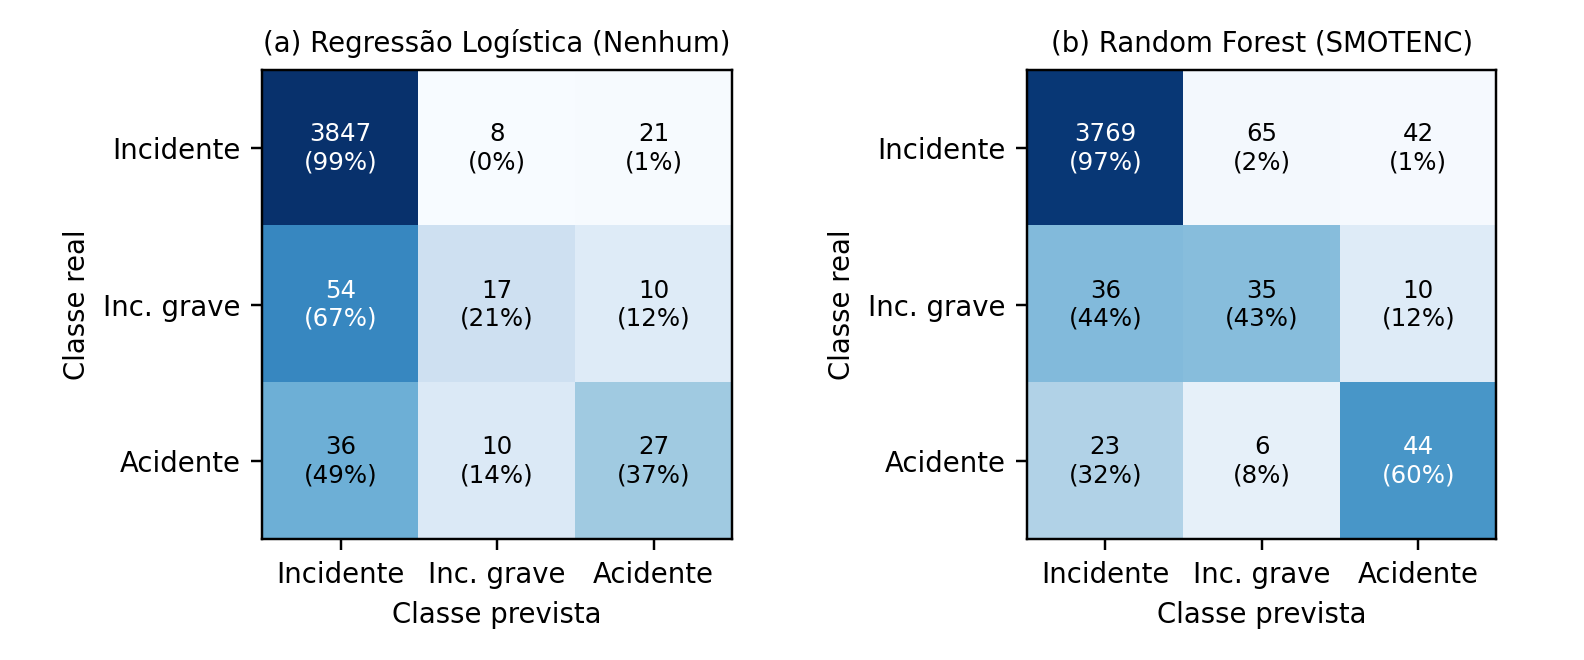
\includegraphics[width=0.6\textwidth]{fig3_confusao.png}
    \caption{Matrizes de confusão das predições \textit{out-of-fold} no treino (contagem e percentual da linha)}
    \label{fig:confusao}
\end{figure}

\begin{figure}[htbp]
    \centering
    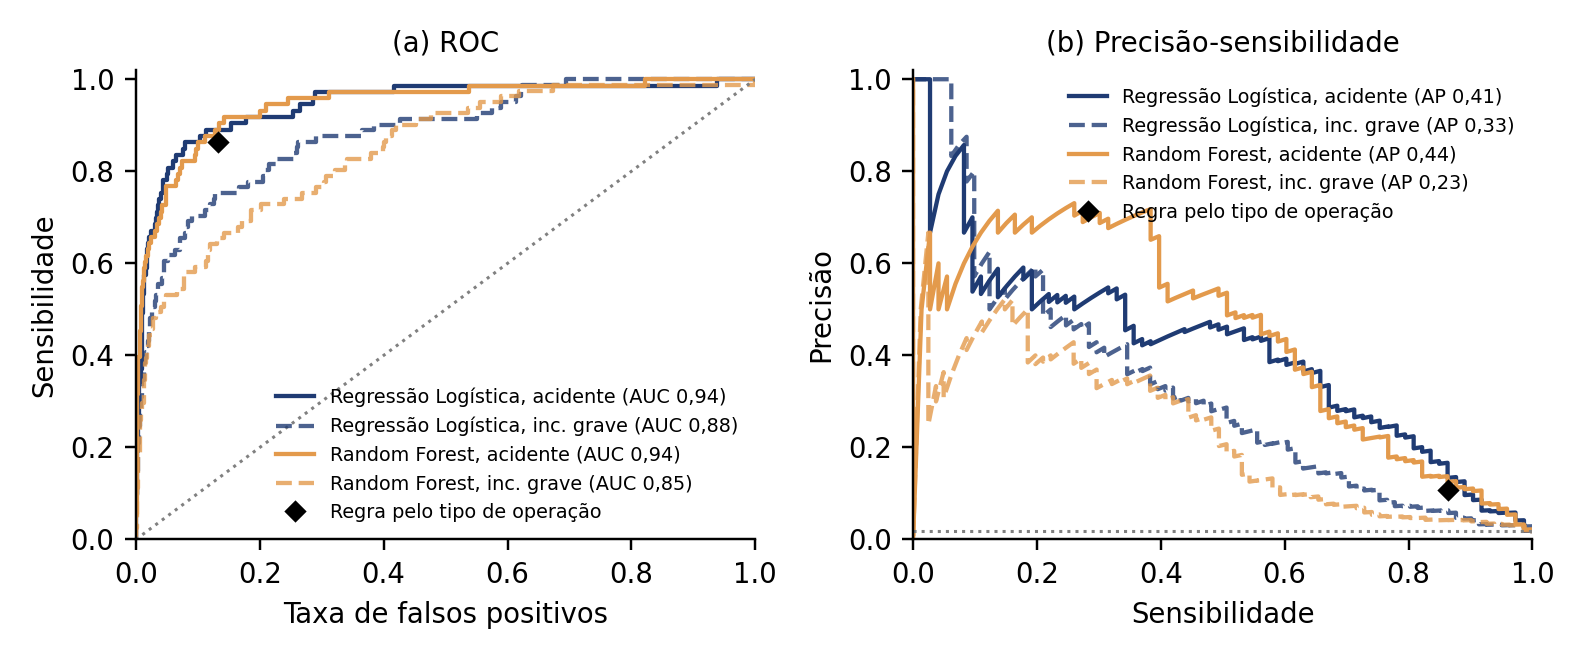
\includegraphics[width=0.72\textwidth]{fig4_curvas.png}
    \caption{Curvas ROC (a) e precisão-sensibilidade (b) um-contra-resto para as classes acidente e incidente grave, predições \textit{out-of-fold} no treino; o losango marca a regra pelo tipo de operação e a linha pontilhada em (b), a prevalência de acidentes}
    \label{fig:curvas}
\end{figure}

\subsection{Interpretação dos modelos}
\label{sec:interpretacao}

A Figura~\ref{fig:importancias} resume o que os modelos aprenderam. Na Regressão Logística (Figura~\ref{fig:importancias}a), os contrastes que mais elevam a chance de acidente em relação a incidente são a categoria perda de controle ou colisão em voo frente à falha técnica (razão de chances da ordem de $10^3$, estimada sobre apenas 20 casos), o fabricante Robinson frente à Airbus (58), o motor turboeixo frente ao jato (48), a ocorrência fora de aeródromo frente aos aeródromos SB (26), as operações não regular (14,9) e de táxi aéreo (14,8) frente à regular e a região Norte frente ao Sudeste (13,3); reduzem a chance a fase de solo (0,01), o helicóptero frente ao avião (0,03) e a colisão com fauna (0,06). Alguns contrastes contrariam as taxas brutas: Cessna, Sikorsky e Embraer aparecem com chance menor que a Airbus, embora suas taxas de acidente sejam maiores. É a colinearidade antecipada na Seção~\ref{sec:operacao}: a taxa marginal desses fabricantes é absorvida pelo tipo de operação, pelo motor e pelo peso, e, com regularização fraca ($C = 10$), os coeficientes individuais tornam-se instáveis e devem ser lidos em conjunto.

O Random Forest (Figura~\ref{fig:importancias}b) atribui as maiores importâncias ao tipo de operação, ao peso máximo de decolagem, à fase do voo, ao local e à categoria do tipo de ocorrência, seguidos pelo número de aeronaves envolvidas, cuja relevância vem dos conflitos de tráfego aéreo com duas aeronaves, típicos dos incidentes graves, e pelo indicador de saída de pista. Mês, dia da semana, hora e número de assentos têm importância nula ou negativa e podem ser removidos na etapa final.

\begin{figure}[htbp]
    \centering
    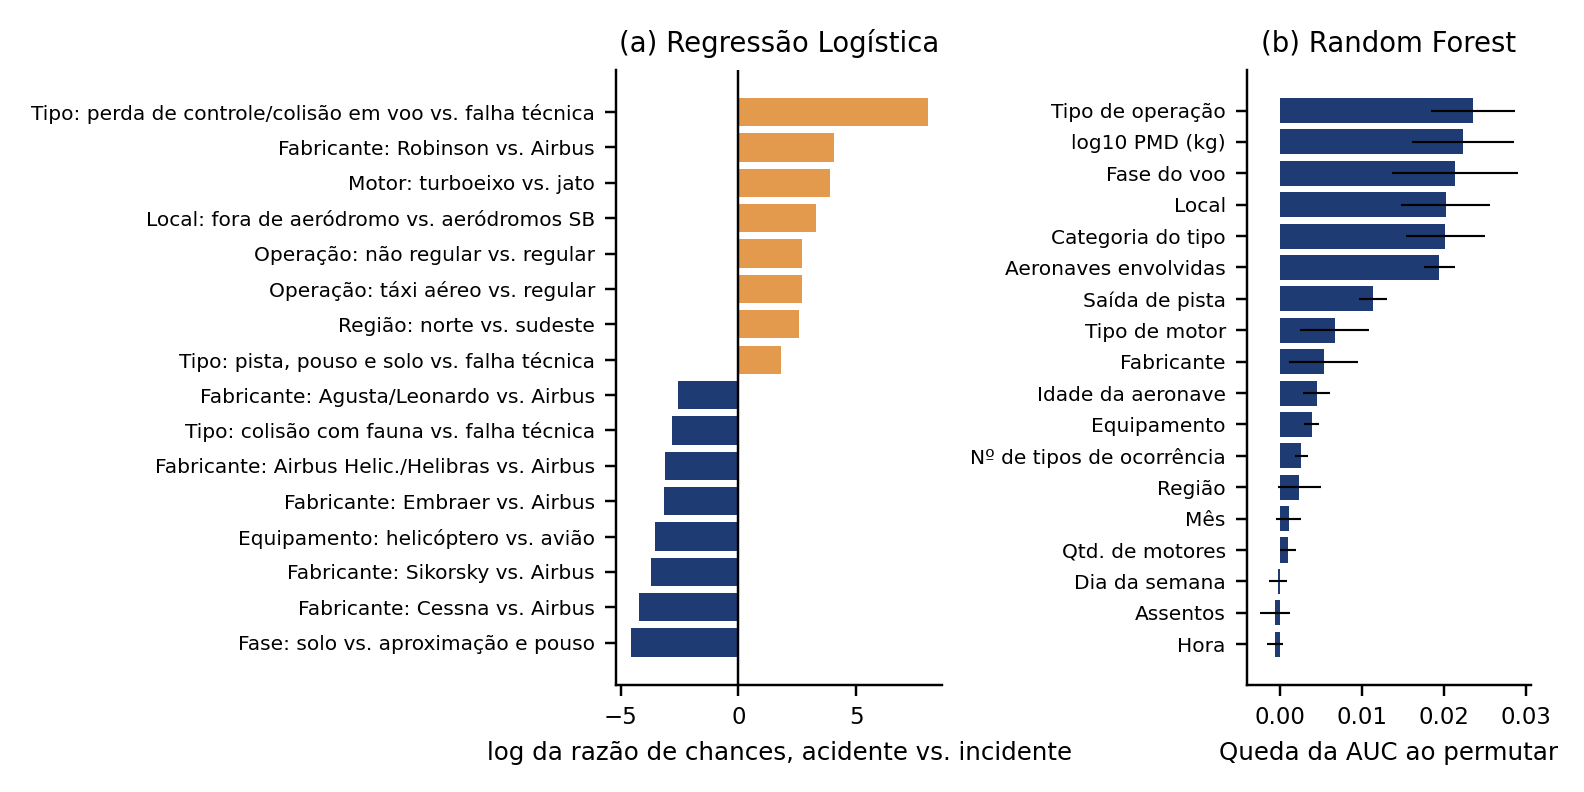
\includegraphics[width=0.76\textwidth]{fig5_importancias.png}
    \caption{(a) Oito maiores e oito menores contrastes de log da razão de chances entre acidente e incidente na Regressão Logística, em relação ao nível mais frequente de cada atributo; (b) importância por permutação no Random Forest, medida pela queda da AUC um-contra-resto no teste (média e desvio-padrão de 30 repetições)}
    \label{fig:importancias}
\end{figure}

\FloatBarrier
\section{Discussão e Conclusão}
\label{sec:conclusao}

Este trabalho construiu, a partir dos dados abertos do CENIPA, uma base de 5.038 ocorrências do transporte aéreo comercial brasileiro e treinou dois algoritmos, Regressão Logística e Random Forest, para classificar a severidade em três classes. Duas decisões estruturaram a modelagem: o alvo com as três classes do CENIPA, justificado pelas definições da NSCA 3-13 e pelos perfis distintos de incidentes graves e acidentes, e o escopo de todo o transporte aéreo comercial, já que a operação regular isolada registra apenas 12 acidentes. É central a exclusão dos atributos produzidos pela investigação, presentes em 92\% dos acidentes, em 44\% a 45\% dos incidentes graves e em 0,1\% dos incidentes.

O Random Forest com SMOTENC foi o melhor modelo, com F1-macro de 0,62, 60\% dos acidentes e 43\% dos incidentes graves detectados fora da amostra e precisão de 46\% para acidentes, resultado confirmado no teste. A Regressão Logística ficou em 0,56 e quase não distingue os incidentes graves, mas foi útil para a interpretação, expondo a colinearidade prevista na análise exploratória. Ambos superam com folga os baselines em F1, mas no mesmo nível de sensibilidade da regra pelo tipo de operação o ganho de precisão é modesto (de 10,7\% para 13,8\% a 16,7\%): os atributos pré-investigação acrescentam informação sobretudo na faixa intermediária de sensibilidade, e o incidente grave, que difere do acidente apenas pela consequência, é a classe mais difícil (AUC de 0,85 a 0,88).

Os resultados têm limitações: o número de acidentes (73 no treino, 18 no teste) produz variância alta, visível na diferença entre as AUC do teste e da validação cruzada; a categoria do tipo de ocorrência descreve parcialmente o desfecho (uma excursão de pista já é uma ocorrência grave) e será avaliada em ablação; e a cobertura das notificações mudou em 2023, sem validação por período (treino até 2022, teste a partir de 2023) até aqui. Os próximos passos, até o relatório final, são: ajustar o limiar de decisão com critério de custo para atingir sensibilidade de ao menos 80\% para acidentes com a melhor precisão possível; remover os atributos de calendário; testar a codificação pelo alvo do aeródromo e do tipo detalhado; estimar intervalos de confiança por validação cruzada repetida; e avaliar a calibração das probabilidades, requisito para que o modelo sirva à priorização de fiscalização e treinamento por reguladores e companhias aéreas.

\bibliographystyle{sbc}
\bibliography{artigo}

\end{document}
